\chapter{Cơ sở lý thuyết}
\label{ch:theory}

\textit{Chương này cung cấp các kiến thức nền tảng về kiến trúc tập lệnh RISC-V, mô hình mạng nơ-ron tích chập (CNN), các chuẩn giao tiếp dữ liệu (AXI, UART, SPI, OSPI, I2C, Camera/HDMI DVP) và công nghệ FPGA được sử dụng trong đề tài.}

\section{Kiến trúc tập lệnh RISC-V}
% Phần này nói về đặc điểm RISC-V, tập lệnh RV32I, Pipeline cơ bản
% File: 2_co_so_ly_thuyet/2.1_kien_truc_riscv.tex

\subsection{Tổng quan về kiến trúc RISC-V}
RISC-V là một kiến trúc tập lệnh (ISA - Instruction Set Architecture) mã nguồn mở, ra đời vào năm 2010 tại Đại học California, Berkeley. Khác với các kiến trúc thương mại phổ biến như x86 (Intel) hay ARM, RISC-V được thiết kế dựa trên nguyên lý máy tính tập lệnh rút gọn (RISC) thuần túy, loại bỏ các gánh nặng tương thích ngược của các kiến trúc cũ để tối ưu hóa hiệu năng và năng lượng.

Đặc điểm cốt lõi của RISC-V là tính mô-đun hóa và khả năng mở rộng. Kiến trúc này không định nghĩa một tập lệnh khổng lồ duy nhất, mà chia thành:
\begin{itemize}
    \item \textbf{Tập lệnh cơ sở (Base ISA):} Là phần cứng tối thiểu bắt buộc phải có để một vi xử lý được gọi là RISC-V. Đối với các ứng dụng nhúng 32-bit, chuẩn này là \textbf{RV32I} (Base Integer). Nó cung cấp đầy đủ các lệnh để thực thi tính toán nguyên, truy cập bộ nhớ và điều khiển luồng chương trình.
    \item \textbf{Các phần mở rộng (Extensions):} Là các mô-đun tùy chọn để tăng cường sức mạnh xử lý. Ví dụ: M (Integer Multiplication/Division), A (Atomic instructions), F (Single-precision Floating-point), C (Compressed instructions - nén lệnh 16-bit để tiết kiệm bộ nhớ).
\end{itemize}
Sự kết hợp này tạo nên chuỗi định danh cho vi xử lý, ví dụ \textbf{RV32IMAC} biểu thị vi xử lý 32-bit có hỗ trợ nhân chia, thao tác nguyên tử và lệnh nén.

\subsection{Mô hình lập trình và Tập thanh ghi}
Theo đặc tả của RV32I, trạng thái kiến trúc của một luồng xử lý (Hart - Hardware Thread) bao gồm hai thành phần chính: bộ đếm chương trình (PC) và tập thanh ghi mục đích chung (GPR).

\subsubsection{Bộ đếm chương trình (Program Counter - PC)}
PC là một thanh ghi 32-bit lưu trữ địa chỉ của lệnh đang được thực thi. Trong RISC-V, PC không phải là một thanh ghi mục đích chung (không thể đánh địa chỉ trực tiếp như GPR). Giá trị của PC chỉ có thể thay đổi thông qua các lệnh rẽ nhánh, nhảy hoặc lệnh hệ thống. Khi khởi động (Reset), PC sẽ được nạp một địa chỉ cố định (Reset Vector) để bắt đầu chu trình nạp lệnh.

\subsubsection{Tập thanh ghi mục đích chung (General Purpose Registers)}
RV32I cung cấp 32 thanh ghi, được đánh số từ \texttt{x0} đến \texttt{x31}, mỗi thanh ghi rộng 32-bit (XLEN=32). Để đảm bảo chương trình phần mềm hoạt động chính xác với phần cứng, đặc biệt khi sử dụng bộ công cụ biên dịch \textbf{RISC-V GNU Toolchain (GCC)}, các thanh ghi này phải tuân thủ chuẩn Giao diện Nhị phân Ứng dụng (ABI - Application Binary Interface). Trình biên dịch GCC sử dụng các tên quy ước (như \texttt{sp}, \texttt{ra}, \texttt{a0}...) thay vì tên phần cứng (\texttt{x2}, \texttt{x1}, \texttt{x10}...) để quản lý việc gọi hàm và truyền tham số. Chi tiết chức năng được trình bày trong Bảng \ref{tab:riscv_registers}.
\begin{table}[H]
    \centering
    \caption{Tập thanh ghi mục đích chung của RISC-V (RV32I)}
    \label{tab:riscv_registers}
    \begin{adjustbox}{width=0.95\textwidth}
    \begin{tabular}{|c|c|l|l|}
        \hline
        \textbf{Tên thanh ghi} & \textbf{Tên ABI} & \textbf{Mô tả chức năng} & \textbf{Lưu bởi} \\ \hline
        \texttt{x0} & \texttt{zero} & Luôn bằng 0 (Hardwired zero) & N/A \\ \hline
        \texttt{x1} & \texttt{ra} & Địa chỉ trả về (Return Address) & Caller \\ \hline
        \texttt{x2} & \texttt{sp} & Con trỏ ngăn xếp (Stack Pointer) & Callee \\ \hline
        \texttt{x3} & \texttt{gp} & Con trỏ toàn cục (Global Pointer) & N/A \\ \hline
        \texttt{x4} & \texttt{tp} & Con trỏ luồng (Thread Pointer) & N/A \\ \hline
        \texttt{x5} & \texttt{t0} & Thanh ghi tạm thời / Địa chỉ trả về thay thế & Caller \\ \hline
        \texttt{x6 - x7} & \texttt{t1 - t2} & Thanh ghi tạm thời (Temporaries) & Caller \\ \hline
        \texttt{x8} & \texttt{s0 / fp} & Thanh ghi lưu trữ / Con trỏ khung (Frame Pointer) & Callee \\ \hline
        \texttt{x9} & \texttt{s1} & Thanh ghi lưu trữ (Saved register) & Callee \\ \hline
        \texttt{x10 - x11} & \texttt{a0 - a1} & Đối số hàm / Giá trị trả về & Caller \\ \hline
        \texttt{x12 - x17} & \texttt{a2 - a7} & Đối số hàm (Function Arguments) & Caller \\ \hline
        \texttt{x18 - x27} & \texttt{s2 - s11} & Thanh ghi lưu trữ (Saved registers) & Callee \\ \hline
        \texttt{x28 - x31} & \texttt{t3 - t6} & Thanh ghi tạm thời (Temporaries) & Caller \\ \hline
    \end{tabular}
    \end{adjustbox}
\end{table}

Trong đó:
\begin{itemize}
    \item \textbf{Caller-saved:} Giá trị không được bảo toàn qua lời gọi hàm (hàm con có thể ghi đè).
    \item \textbf{Callee-saved:} Giá trị phải được bảo toàn (nếu hàm con muốn dùng, phải lưu ra stack trước và khôi phục lại trước khi return).
\end{itemize}

\subsection{Đặc tả tập lệnh cơ sở RV32I}
Tập lệnh RV32I bao gồm 47 lệnh cơ bản. Một điểm đặc biệt trong thiết kế của RISC-V là việc cố định độ dài lệnh ở 32-bit và căn chỉnh bộ nhớ theo từ (word-aligned), giúp đơn giản hóa mạch giải mã lệnh và dự đoán rẽ nhánh.

\subsubsection{Định dạng lệnh (Instruction Formats)}
RISC-V sử dụng 6 định dạng lệnh cơ bản (R, I, S, B, U, J). Điểm tối ưu trong thiết kế định dạng lệnh của RISC-V là vị trí của các trường thanh ghi nguồn (\texttt{rs1}, \texttt{rs2}) và thanh ghi đích (\texttt{rd}) luôn được giữ cố định tại các bit giống nhau trong mọi định dạng lệnh (xem Hình \ref{fig:rv32i_formats}).

Điều này cho phép bộ giải mã (Decoder) có thể bắt đầu đọc dữ liệu từ tập thanh ghi (Register File) ngay lập tức mà không cần phải chờ xác định xong loại lệnh (Opcode), giúp giảm độ trễ trong đường ống xử lý.

\begin{figure}[H]
    \centering
    \begin{tabular}{|c|c|c|c|c|c|c|}
        \hline
        \textbf{Bit} & \textbf{31...25} & \textbf{24...20} & \textbf{19...15} & \textbf{14...12} & \textbf{11...7} & \textbf{6...0} \\ \hline
        R-type & funct7 & rs2 & rs1 & funct3 & rd & opcode \\ \hline
        I-type & \multicolumn{2}{c|}{imm[11:0]} & rs1 & funct3 & rd & opcode \\ \hline
        S-type & imm[11:5] & rs2 & rs1 & funct3 & imm[4:0] & opcode \\ \hline
        B-type & imm[12|10:5] & rs2 & rs1 & funct3 & imm[4:1|11] & opcode \\ \hline
        U-type & \multicolumn{4}{c|}{imm[31:12]} & rd & opcode \\ \hline
        J-type & \multicolumn{4}{c|}{imm[20|10:1|11|19]} & rd & opcode \\ \hline
    \end{tabular}
    \caption{Cấu trúc bit của các định dạng lệnh RV32I}
    \label{fig:rv32i_formats}
\end{figure}

Dưới đây là giải thích chi tiết ý nghĩa của từng loại định dạng lệnh:
\begin{itemize}
    \item \textbf{R-type (Register):} Dùng cho các lệnh thao tác trực tiếp giữa thanh ghi và thanh ghi (ví dụ: \texttt{add x1, x2, x3}).
    \item \textbf{I-type (Immediate):} Dùng cho các lệnh thao tác với hằng số ngắn (Immediate) và các lệnh nạp dữ liệu (Load) từ bộ nhớ.
    \item \textbf{S-type (Store):} Dùng chuyên biệt cho các lệnh lưu dữ liệu từ thanh ghi vào bộ nhớ.
    \item \textbf{B-type (Branch):} Dùng cho các lệnh rẽ nhánh có điều kiện (ví dụ: so sánh bằng, so sánh lớn hơn).
    \item \textbf{U-type (Upper Immediate):} Dùng để thao tác với các hằng số lớn (20-bit cao), thường dùng để nạp địa chỉ nền.
    \item \textbf{J-type (Jump):} Dùng cho các lệnh nhảy vô điều kiện (dùng trong gọi hàm hoặc vòng lặp).
\end{itemize}

Một kỹ thuật quan trọng khác là việc mã hóa giá trị tức thời (Immediate Encoding). Trong các lệnh dạng S và B, các bit giá trị tức thời bị phân mảnh và xáo trộn. Tuy nhiên, việc xáo trộn này được thiết kế có chủ đích để các bit này luôn tương ứng với cùng một vị trí bit đầu ra của bộ tạo giá trị tức thời (Immediate Generator), giúp giảm số lượng tầng logic (Fan-out) trong phần cứng.

\subsubsection{Phân nhóm chức năng chi tiết}

\textbf{1. Lệnh tính toán số nguyên (Integer Computational Instructions):} \\
Nhóm lệnh này thực hiện các phép toán số học và logic. Chúng không gây ra ngoại lệ số học và không thay đổi bất kỳ cờ trạng thái nào (RISC-V không sử dụng thanh ghi cờ như ARM/x86).
\begin{itemize}
    \item \textbf{Tính toán với hằng số (I-Type):} \texttt{ADDI}, \texttt{ANDI}, \texttt{ORI}, \texttt{XORI}, \texttt{SLTI} (Set Less Than Immediate). Lệnh \texttt{LUI} (Load Upper Immediate) dùng để nạp 20-bit cao vào thanh ghi.
    \item \textbf{Tính toán giữa các thanh ghi (R-Type):} \texttt{ADD}, \texttt{SUB}, \texttt{AND}, \texttt{OR}, \texttt{XOR}. Lệnh \texttt{SLT/SLTU} so sánh hai thanh ghi và ghi giá trị 1 vào đích nếu nhỏ hơn, ngược lại ghi 0.
    \item \textbf{Dịch bit:} \texttt{SLL/SLLI} (Dịch trái logic), \texttt{SRL/SRLI} (Dịch phải logic - chèn 0), \texttt{SRA/SRAI} (Dịch phải số học - giữ nguyên dấu).
\end{itemize}

\textbf{2. Lệnh truy cập bộ nhớ (Load and Store Instructions):} \\
RISC-V sử dụng kiến trúc Load-Store thuần túy. Việc tính toán địa chỉ bộ nhớ luôn thông qua công thức: $Address = rs1 + sign\_extend(imm)$.
\begin{itemize}
    \item \textbf{Load:} \texttt{LW} (32-bit), \texttt{LH} (16-bit), \texttt{LB} (8-bit). Các biến thể \texttt{LHU} và \texttt{LBU} dùng để nạp dữ liệu không dấu, trong đó phần bit cao của thanh ghi đích sẽ được điền 0 (Zero-extension) thay vì mở rộng dấu (Sign-extension).
    \item \textbf{Store:} \texttt{SW}, \texttt{SH}, \texttt{SB}. Lệnh store chỉ lấy các bit thấp tương ứng trong thanh ghi nguồn để ghi vào bộ nhớ.
\end{itemize}

\textbf{3. Lệnh điều khiển luồng (Control Transfer Instructions):} \\
RISC-V khác biệt so với các kiến trúc cũ ở chỗ lệnh rẽ nhánh thực hiện so sánh trực tiếp hai thanh ghi.
\begin{itemize}
    \item \textbf{Rẽ nhánh có điều kiện (Branch):} \texttt{BEQ} (Bằng), \texttt{BNE} (Không bằng), \texttt{BLT/BGE} (So sánh có dấu), \texttt{BLTU/BGEU} (So sánh không dấu). Việc tách biệt so sánh có dấu và không dấu giúp lập trình viên kiểm soát chính xác các cấu trúc điều khiển.
    \item \textbf{Nhảy vô điều kiện (Jump):} 
    \begin{itemize}
        \item[] \texttt{JAL} (Jump and Link): Nhảy đến địa chỉ tương đối so với PC, đồng thời lưu địa chỉ lệnh kế tiếp (PC+4) vào thanh ghi \texttt{rd} (thường là \texttt{ra}).
        \item[] \texttt{JALR} (Jump and Link Register): Nhảy đến địa chỉ tuyệt đối được tính từ thanh ghi cơ sở + offset. Lệnh này hỗ trợ việc gọi hàm qua con trỏ hoặc quay về từ hàm (Return).
    \end{itemize}
\end{itemize}

\textbf{4. Lệnh môi trường hệ thống (System Environment):} \\
Hai lệnh quan trọng nhất là \texttt{ECALL} (Environment Call) dùng để tạo yêu cầu phục vụ từ hệ điều hành (System Call) và \texttt{EBREAK} (Environment Break) dùng để chuyển quyền kiểm soát cho trình gỡ lỗi (Debugger). Ngoài ra, các lệnh \texttt{CSRRW, CSRRS, CSRRC} dùng để đọc/ghi các thanh ghi trạng thái điều khiển (CSR) nhằm quản lý ngắt và cấu hình hệ thống.

\subsection{Vi xử lý PicoRV32}
Trong đồ án này, nhóm thực hiện lựa chọn lõi vi xử lý \textbf{PicoRV32} để làm bộ xử lý trung tâm cho hệ thống SoC.

PicoRV32 là một hiện thực phần cứng (CPU Core) của kiến trúc RISC-V, hỗ trợ đầy đủ tập lệnh cơ sở \textbf{RV32I}. Đặc điểm nổi bật của PicoRV32 là sự tối ưu hóa về mặt diện tích và tài nguyên trên FPGA, thay vì tập trung vào hiệu năng đường ống (Pipeline) phức tạp. Nó hoạt động dựa trên máy trạng thái đa chu kỳ, cho phép đạt tần số hoạt động cao và dễ dàng tích hợp vào các thiết kế SoC nhỏ gọn phục vụ ứng dụng IoT. Ngoài ra, PicoRV32 cung cấp giao diện đồng xử lý (PCPI), cho phép mở rộng khả năng tính toán thông qua các bộ tăng tốc phần cứng bên ngoài.

\section{Tổng quan về Mạng nơ-ron tích chập (CNN)}
% Phần này nói về Convolution, Pooling, ReLU, Fully Connected


Phần này trình bày các cơ sở lý thuyết về trí tuệ nhân tạo, trọng tâm là các mạng nơ-ron tích chập (CNN). Đồng thời, các phân tích về xu hướng tính toán biên (Edge AI) và đặc tả toán học của các phép tính cốt lõi cũng được thảo luận chi tiết nhằm làm rõ động lực thiết kế phần cứng của đồ án.

\subsection{Trí tuệ nhân tạo và Học sâu}

Trí tuệ nhân tạo (Artificial Intelligence - AI) là lĩnh vực khoa học kỹ thuật với mục tiêu kiến tạo các hệ thống máy móc thông minh, sở hữu khả năng thực hiện các tác vụ vốn đòi hỏi trí tuệ con người. Là một tập con quan trọng của AI, Học máy (Machine Learning - ML) cho phép máy tính tự học hỏi từ dữ liệu và cải thiện hiệu suất mà không cần lập trình cụ thể cho từng tác vụ. Thay vì dựa vào các quy tắc thủ công tĩnh, các thuật toán ML sử dụng quá trình huấn luyện để xây dựng mô hình giải quyết vấn đề.

Trong đó, Học sâu (Deep Learning - DL) là bước tiến vượt bậc của ML, tập trung phát triển các Mạng nơ-ron sâu (Deep Neural Networks - DNNs). Các mạng hiện đại có thể sở hữu từ 5 đến hàng nghìn lớp, vượt xa quy mô của các mạng nơ-ron truyền thống. Sức mạnh vượt trội của DNN nằm ở khả năng phân cấp đặc trưng (Feature Hierarchy). Khi dữ liệu đi qua các lớp của mạng, thông tin được trích xuất theo mức độ trừu tượng tăng dần: từ các đặc trưng cấp thấp như cạnh, đường thẳng ở lớp đầu, đến hình dạng phức tạp ở lớp giữa, và cuối cùng là nhận diện vật thể hoàn chỉnh ở lớp cuối. Cấu trúc này đặc biệt hiệu quả trong các bài toán Thị giác máy tính (Computer Vision) như phân loại ảnh hay xe tự hành.

\subsection{Xu hướng chuyển dịch tính toán xuống biên (Edge AI)}

Vòng đời của một mô hình AI bao gồm hai giai đoạn chính là Huấn luyện (Training) và Suy luận (Inference). Trong khi quá trình huấn luyện đòi hỏi tài nguyên khổng lồ thường thực hiện trên Cloud, quá trình suy luận đang có xu hướng dịch chuyển mạnh mẽ xuống các thiết bị biên (Edge devices/IoT).

Việc đưa tác vụ Inference xuống biên, hay còn gọi là Edge AI, giải quyết được ba thách thức cốt lõi của mô hình tập trung. Thứ nhất là độ trễ (latency), yếu tố sống còn đối với các ứng dụng thời gian thực như xe tự lái, nơi độ trễ đường truyền Cloud có thể gây rủi ro an toàn. Thứ hai là tối ưu hóa băng thông mạng khi không cần truyền tải dữ liệu thô (như video giám sát) lên máy chủ. Cuối cùng là đảm bảo quyền riêng tư và bảo mật dữ liệu người dùng.

Tuy nhiên, các nền tảng nhúng thường bị giới hạn nghiêm ngặt về ngân sách năng lượng, tài nguyên tính toán và dung lượng bộ nhớ. Do đó, việc thiết kế các kiến trúc phần cứng chuyên dụng (AI Accelerator) để xử lý hiệu quả các thuật toán DNN dưới các ràng buộc này là yêu cầu cấp thiết.

\subsection{Cơ sở toán học của Mạng Nơ-ron Tích chập (CNN)}

Mạng nơ-ron tích chập (CNN) là kiến trúc phổ biến nhất trong Deep Learning để xử lý dữ liệu hình ảnh. Để đảm bảo tính linh hoạt cho phần cứng, đồ án tập trung phân tích đặc tả toán học của hai loại phép tính cốt lõi thường gặp: Standard Convolution và Depthwise Separable Convolution.

\subsubsection{Standard Convolution (Tích chập tiêu chuẩn)}
Standard Convolution thực hiện trượt bộ lọc trên không gian đầu vào và tích lũy giá trị qua toàn bộ chiều sâu kênh (Channels). Giá trị đầu ra $O$ tại kênh $m$, vị trí $(h, w)$ được xác định bởi công thức:

\begin{equation}
    O[m][h][w] = B[m] + \sum_{c=0}^{C-1} \sum_{r=0}^{R-1} \sum_{s=0}^{S-1} I[c][h \cdot U + r - P][w \cdot U + s - P] \times W[m][c][r][s]
    \label{eq:std_conv}
\end{equation}

Trong đó, $U$ là bước trượt (Stride), $P$ là lượng đệm (Padding), $W$ là trọng số và $I$ là đầu vào. Việc xử lý biên (Padding) đóng vai trò quan trọng để duy trì kích thước không gian, yêu cầu phần cứng phải có logic tự động chèn giá trị 0 (Zero-padding) khi chỉ số truy cập nằm ngoài phạm vi hình ảnh thực tế.

\subsubsection{Depthwise Separable Convolution}
Để tối ưu hóa cho các thiết bị biên có tài nguyên hạn chế, các kiến trúc hiện đại như MobileNet sử dụng kỹ thuật Depthwise Separable Convolution. Kỹ thuật này tách tích chập chuẩn thành hai bước riêng biệt nhằm giảm đáng kể khối lượng tính toán:

\textbf{1. Depthwise Convolution (DW):} Áp dụng bộ lọc riêng biệt cho từng kênh đầu vào mà không tích lũy qua các kênh. Do tính độc lập giữa các kênh, các đơn vị tính toán có thể hoạt động song song hoàn toàn.
\begin{equation}
    O_{dw}[c][h][w] = \sum_{r=0}^{R-1} \sum_{s=0}^{S-1} I[c][h \cdot U + r - P][w \cdot U + s - P] \times W_{dw}[c][r][s]
\end{equation}

\textbf{2. Pointwise Convolution (PW):} Là tích chập chuẩn với kích thước kernel $1 \times 1$, thực hiện nhiệm vụ trộn thông tin giữa các kênh (channel mixing).
\begin{equation}
    O_{pw}[m][h][w] = \sum_{c=0}^{C-1} I[c][h][w] \times W_{pw}[m][c]
\end{equation}

Từ phân tích trên, kiến trúc phần cứng đề xuất cần có khả năng cấu hình linh hoạt (reconfigurable) để hỗ trợ cả chế độ tích lũy theo không gian (cho Standard/Pointwise) và chế độ tính toán độc lập theo kênh (cho Depthwise).

\subsection{Kỹ thuật Gập Batch Normalization (BN Folding)}

Trong giai đoạn suy luận, để giảm thiểu độ phức tạp tính toán, đồ án áp dụng kỹ thuật BN Folding. Lớp Batch Normalization thường đi kèm sau Convolution có các tham số $(\mu, \sigma, \gamma, \beta)$ là hằng số cố định khi suy luận. Ta có thể gộp các phép tính này vào trực tiếp trọng số ($W$) và bias ($B$) của lớp Convolution phía trước:

\begin{equation}
    W' = W_{orig} \cdot \frac{\gamma}{\sqrt{\sigma^2 + \epsilon}}; \quad B' = \left( B_{orig} - \mu \right) \cdot \frac{\gamma}{\sqrt{\sigma^2 + \epsilon}} + \beta
\end{equation}

Kỹ thuật này giúp loại bỏ hoàn toàn khối tính toán Batch Normalization trên phần cứng, giúp tiết kiệm tài nguyên và giảm độ trễ xử lý mà không làm ảnh hưởng đến độ chính xác của mô hình.

\subsection{Mô hình và Dữ liệu kiểm thử}

Để đánh giá hiệu năng hệ thống, đồ án sử dụng các mô hình đã huấn luyện sẵn (Pretrained Models) được chuẩn hóa qua định dạng ONNX. Các bộ dữ liệu kiểm thử bao gồm MNIST (nhận diện chữ số), CIFAR-10 (phân loại vật thể cơ bản) và ImageNet. Trong đó, ImageNet với 1000 lớp vật thể là chuẩn mực quan trọng để đánh giá độ chính xác Top-1 và Top-5 của các mạng nơ-ron sâu hiện đại.

\section{Các chuẩn giao tiếp hệ thống}
% Phần này nói về AXI4/AXI-Lite, UART, SPI, DVP
    % File: 2_co_so_ly_thuyet/2.3_chuan_giao_tiep.tex

    \subsection{Chuẩn giao tiếp AMBA AXI4}
    AMBA (Advanced Microcontroller Bus Architecture) là tiêu chuẩn kết nối trên chip (On-Chip Interconnect) phổ biến nhất hiện nay, được phát triển bởi ARM. Trong đó, giao thức AXI (Advanced eXtensible Interface) là chuẩn giao tiếp hiệu năng cao, được thiết kế cho các hệ thống SoC yêu cầu băng thông lớn và độ trễ thấp.

    Phiên bản AXI4 (được giới thiệu trong AMBA 4.0) hỗ trợ các tính năng vượt trội so với các thế hệ trước:
    \begin{itemize}
        \item Tách biệt hoàn toàn pha địa chỉ/điều khiển và pha dữ liệu.
        \item Hỗ trợ giao dịch dữ liệu không thẳng hàng (Unaligned data transfers).
        \item Cho phép phát hành nhiều địa chỉ chờ (Outstanding addresses) trước khi dữ liệu hoàn tất.
        \item Hỗ trợ hoàn thành giao dịch không theo thứ tự (Out-of-order completion) thông qua ID.
    \end{itemize}

    \begin{figure}[H]
        \centering
        \includegraphics[width=0.5\linewidth]{2_co_so_ly_thuyet/image/axi.png} 
        \caption{a. Tổng quan giao thức AXI4}
        \label{fig:axi_channels}
    \end{figure}

    \begin{figure}[H]
        \centering
        \includegraphics[width=0.9\linewidth]{2_co_so_ly_thuyet/image/axi2.png} 
        \caption{b. Tổng quan giao thức AXI4}
        \label{fig:axi_channels}
    \end{figure}



    \subsubsection{Kiến trúc 5 kênh độc lập (Channel Architecture)}
    AXI chia nhỏ một giao dịch truyền thông thành 5 kênh riêng biệt hoạt động song song. Kiến trúc này cho phép đường truyền dữ liệu hai chiều (Full-duplex), nghĩa là Master có thể ghi dữ liệu vào Slave trong khi đang đọc dữ liệu từ Slave khác.

    \begin{figure}[H]
        \centering
        \includegraphics[width=0.9\linewidth]{2_co_so_ly_thuyet/image/axichannel.png} 
        \caption{Mô hình 5 kênh giao tiếp của AXI4}
        \label{fig:axi_channels}
    \end{figure}

    Năm kênh tín hiệu bao gồm:
    \begin{enumerate}
        \item \textbf{Write Address Channel (AW):} Master gửi địa chỉ bắt đầu và thông tin điều khiển (loại burst, độ dài) cho giao dịch ghi. Các tín hiệu bắt đầu bằng \texttt{AW...} (ví dụ: \texttt{AWADDR}, \texttt{AWVALID}).
        \item \textbf{Write Data Channel (W):} Master truyền dữ liệu thực tế tới Slave. Kênh này hỗ trợ tín hiệu \texttt{WSTRB} (Strobe) để đánh dấu các byte hợp lệ trong một word (hỗ trợ ghi từng byte). Các tín hiệu bắt đầu bằng \texttt{W...}.
        \item \textbf{Write Response Channel (B):} Slave gửi phản hồi trạng thái (OKAY, ERROR) cho Master sau khi toàn bộ dữ liệu đã được ghi thành công. Tín hiệu bắt đầu bằng \texttt{B...}.
        \item \textbf{Read Address Channel (AR):} Master gửi địa chỉ bắt đầu cho giao dịch đọc. Tín hiệu bắt đầu bằng \texttt{AR...}.
        \item \textbf{Read Data Channel (R):} Slave trả về dữ liệu yêu cầu cùng với trạng thái đọc. Tín hiệu bắt đầu bằng \texttt{R...}.
    \end{enumerate}

    \subsubsection{Cơ chế bắt tay (Handshake Mechanism)}
    Toàn bộ 5 kênh AXI đều sử dụng chung một cơ chế bắt tay hai chiều \texttt{VALID/READY} để điều khiển luồng dữ liệu:
    \begin{itemize}
        \item \textbf{VALID (từ Bên gửi):} Báo hiệu rằng dữ liệu hoặc địa chỉ trên đường truyền đã hợp lệ và ổn định.
        \item \textbf{READY (từ Bên nhận):} Báo hiệu rằng bên nhận đã sẵn sàng chấp nhận dữ liệu mới.
    \end{itemize}

    \begin{figure}[H]
        \centering
        \includegraphics[width=0.9\linewidth]{2_co_so_ly_thuyet/image/battay.png} 
        \caption{Cơ chế bắt tay VALID/READY trong AXI}
        \label{fig:axi_handshake}
    \end{figure}

    Giao dịch chỉ thực sự diễn ra tại cạnh dương của xung nhịp khi và chỉ khi cả \texttt{VALID} và \texttt{READY} đều ở mức cao (High). Cơ chế này cho phép bên nhận có thể "kìm" (back-pressure) bên gửi nếu bộ đệm bị đầy, hoặc bên gửi có thể đợi chuẩn bị dữ liệu xong mới phát tín hiệu.

    Dựa trên cơ chế bắt tay này, chuẩn AXI định nghĩa hai cấp độ truyền tải dữ liệu cần phân biệt rõ:
    \begin{itemize}
        \item \textbf{Transfer (hoặc Beat):} Là một lần trao đổi dữ liệu đơn lẻ thành công (một lần bắt tay VALID/READY = 1). Trong một chuỗi dữ liệu (Burst), mỗi nhịp truyền một gói tin (ví dụ 32-bit) được gọi là một Transfer.
        
        \begin{figure}[H]
            \centering
            \includegraphics[width=0.9\linewidth]{2_co_so_ly_thuyet/image/transfer.png} 
            \caption{Minh họa một Transfer trong AXI}
            \label{fig:axi_handshake}
        \end{figure}

        \item \textbf{Transaction (Giao dịch):} Là một hoạt động đọc hoặc ghi hoàn chỉnh. Một Transaction bao gồm toàn bộ quá trình: gửi địa chỉ (Address Phase), truyền một hoặc nhiều dữ liệu (Data Phase - gồm nhiều Transfers) và nhận phản hồi (Response Phase).
        \begin{figure}[H]
            \centering
            \includegraphics[width=0.9\linewidth]{2_co_so_ly_thuyet/image/transaction.png} 
            \caption{Minh họa một Transaction trong AXI}
            \label{fig:axi_handshake}
        \end{figure}

    \end{itemize}

    % --- ĐOẠN BỔ SUNG VÀO SAU PHẦN TRANSFER/TRANSACTION ---% --- THAY THẾ CHO MỤC QUY TRÌNH GIAO DỊCH CŨ ---

    \subsubsection{Quy trình thực hiện giao dịch chi tiết (Transaction Steps)}
    Để đảm bảo toàn vẹn dữ liệu, chuẩn AXI quy định chặt chẽ về hướng đi của tín hiệu và trình tự bắt tay giữa Master và Slave. Dưới đây là mô tả chi tiết các tín hiệu tham gia vào hai loại giao dịch cơ bản.

    \textbf{1. Giao dịch Ghi (Write Transaction)} \\
    Quá trình ghi dữ liệu diễn ra qua 3 pha, sử dụng các kênh AW, W và B.

    \begin{figure}[H]
        \centering
        \includegraphics[width=0.9\linewidth]{2_co_so_ly_thuyet/image/write.png} 
        \caption{Giản đồ tín hiệu chi tiết của giao dịch Ghi}
        \label{fig:axi_write_trans}
    \end{figure}

    \begin{itemize}
        \item \textbf{Pha địa chỉ (Write Address Channel):}
        \begin{itemize}
            \item \textbf{Master $\rightarrow$ Slave:} Master đặt địa chỉ lên bus \texttt{AWADDR} và các thông tin điều khiển (Burst type, length) lên \texttt{AWLEN}, \texttt{AWSIZE}... sau đó xác lập tín hiệu \texttt{AWVALID = 1}.
            \item \textbf{Slave $\rightarrow$ Master:} Khi Slave sẵn sàng nhận địa chỉ, nó bật \texttt{AWREADY = 1}. Giao dịch địa chỉ hoàn tất.
        \end{itemize}
        
        \item \textbf{Pha dữ liệu (Write Data Channel):}
        \begin{itemize}
            \item \textbf{Master $\rightarrow$ Slave:} Master đưa dữ liệu lên bus \texttt{WDATA}. Nếu đây là gói cuối cùng trong Burst, Master bật tín hiệu \texttt{WLAST = 1}. Đồng thời, Master xác lập \texttt{WVALID = 1}.
            \item \textbf{Slave $\rightarrow$ Master:} Slave bật \texttt{WREADY = 1} để báo hiệu đã nhận gói dữ liệu đó. Quá trình lặp lại cho đến hết Burst.
        \end{itemize}

        \item \textbf{Pha phản hồi (Write Response Channel):}
        \begin{itemize}
            \item \textbf{Slave $\rightarrow$ Master:} Sau khi nhận đủ dữ liệu và hoàn tất việc ghi vào bộ nhớ, Slave gửi trạng thái (ví dụ: OKAY) qua bus \texttt{BRESP} và xác lập \texttt{BVALID = 1}.
            \item \textbf{Master $\rightarrow$ Slave:} Master xác nhận đã nhận được phản hồi bằng cách bật \texttt{BREADY = 1}. Kết thúc giao dịch.
        \end{itemize}
    \end{itemize}

    \textbf{2. Giao dịch Đọc (Read Transaction)} \\
    Quá trình đọc dữ liệu diễn ra qua 2 pha, sử dụng kênh AR và R.

    \begin{figure}[H]
        \centering
        \includegraphics[width=0.9\linewidth]{2_co_so_ly_thuyet/image/read.png} 
        \caption{Giản đồ tín hiệu chi tiết của giao dịch Đọc}
        \label{fig:axi_read_trans}
    \end{figure}

    \begin{itemize}
        \item \textbf{Pha địa chỉ (Read Address Channel):}
        \begin{itemize}
            \item \textbf{Master $\rightarrow$ Slave:} Master đặt địa chỉ cần đọc lên bus \texttt{ARADDR} cùng các tham số điều khiển, sau đó bật \texttt{ARVALID = 1}.
            \item \textbf{Slave $\rightarrow$ Master:} Slave chấp nhận địa chỉ bằng cách bật \texttt{ARREADY = 1}.
        \end{itemize}

        \item \textbf{Pha dữ liệu (Read Data Channel):}
        \begin{itemize}
            \item \textbf{Slave $\rightarrow$ Master:} Slave truy xuất dữ liệu và đưa lên bus \texttt{RDATA}. Nếu thành công, Slave gửi kèm trạng thái OKAY trên bus \texttt{RRESP}. Tại gói dữ liệu cuối cùng, Slave bật \texttt{RLAST = 1}. Tín hiệu \texttt{RVALID = 1} được xác lập khi dữ liệu trên bus là hợp lệ.
            \item \textbf{Master $\rightarrow$ Slave:} Master nhận dữ liệu bằng cách bật \texttt{RREADY = 1}.
        \end{itemize}
    \end{itemize}
    
    % --- HẾT PHẦN BỔ SUNG ---


    \subsubsection{Cấu trúc giao dịch Burst (Burst Transaction)}
    AXI là giao thức dựa trên Burst, nghĩa là chỉ cần gửi một địa chỉ khởi đầu, Master có thể truyền liên tiếp một chuỗi dữ liệu (tức là thực hiện một Transaction gồm nhiều Transfers). Các tham số chính điều khiển Burst bao gồm:

    \begin{itemize}
        \item \textbf{Burst Length (AxLEN):} Số lượng gói dữ liệu (beat/transfer) trong một burst. AXI4 hỗ trợ lên đến 256 beat cho kiểu INCR.
        \item \textbf{Burst Size (AxSIZE):} Số byte trong mỗi beat (ví dụ: 4 bytes cho hệ thống 32-bit).
        \item \textbf{Burst Type (AxBURST):} Xác định cách tính địa chỉ cho các beat tiếp theo:
        \begin{itemize}
            \item \textit{FIXED:} Địa chỉ giữ nguyên (dùng cho FIFO).
            \item \textit{INCR (Incrementing):} Địa chỉ tăng dần (dùng cho RAM). Đây là kiểu phổ biến nhất.
            \item \textit{WRAP:} Địa chỉ tăng đến giới hạn biên rồi quay vòng (dùng cho Cache Line fill).
        \end{itemize}
    \end{itemize}

    \subsubsection{Các biến thể giao thức trong thiết kế}
    Trong phiên bản AXI4, chuẩn AMBA định nghĩa thêm các biến thể rút gọn để phù hợp với từng mục đích sử dụng cụ thể:

    \textbf{1. Giao thức AXI4-Lite (AXI-Lite)} \\
    AXI4-Lite là một phiên bản rút gọn của AXI4, được thiết kế cho các giao tiếp điều khiển đơn giản, không yêu cầu truyền dữ liệu tốc độ cao (Burst transfer). Đặc điểm chính của AXI4-Lite bao gồm:
    \begin{itemize}
        \item Mỗi giao dịch chỉ truyền một gói dữ liệu đơn lẻ (Burst length = 1).
        \item Dữ liệu thường có độ rộng 32-bit hoặc 64-bit cố định.
        \item Đơn giản hóa logic điều khiển, giảm diện tích phần cứng.
    \end{itemize}
    Nhờ sự đơn giản này, AXI4-Lite thường được sử dụng làm giao diện cấu hình cho các thanh ghi điều khiển (Control Registers) bên trong các khối IP (Intellectual Property).

    \textbf{2. Giao thức AXI4-Stream (AXI-Stream)} \\
    AXI4-Stream được thiết kế chuyên biệt cho việc truyền tải các luồng dữ liệu liên tục tốc độ cao (Streaming data) mà không cần sử dụng địa chỉ. Khác với AXI4-Lite hay AXI4-Full (Memory Mapped), AXI4-Stream chỉ tập trung vào việc đẩy dữ liệu từ nguồn (Master) đến đích (Slave) nhanh nhất có thể.
    \begin{itemize}
        \item Không có kênh địa chỉ (Address Channel), giảm đáng kể số lượng dây tín hiệu.
        \item Hỗ trợ truyền dữ liệu liên tục không giới hạn độ dài Burst.
        \item Thích hợp cho dữ liệu video, âm thanh hoặc dữ liệu mạng nơ-ron (Feature maps).
    \end{itemize}

    \subsubsection{Áp dụng trong hệ thống đề tài}
    Trong khuôn khổ đồ án thiết kế SoC RISC-V tích hợp EdgeAI này, nhóm thực hiện áp dụng kết hợp cả hai chuẩn giao tiếp trên để tối ưu hóa hiệu năng và tài nguyên:

    \begin{itemize}
        \item \textbf{Sử dụng AXI4-Lite:} Đóng vai trò là kênh điều khiển (Control Plane). Vi xử lý PicoRV32 (Master) sẽ sử dụng AXI4-Lite để ghi vào các thanh ghi cấu hình của khối ngoại vi, khối Accelerator và DMA, thiết lập các thông số như kích thước ảnh, địa chỉ bộ nhớ và tín hiệu bắt đầu (Start).
        \item \textbf{Sử dụng AXI4-Stream:} Đóng vai trò là kênh dữ liệu (Data Plane). Dữ liệu hình ảnh từ Camera và các ma trận trọng số (Weights) sẽ được truyền trực tiếp từ DMA vào khối Accelerator thông qua AXI4-Stream. Việc loại bỏ overhead của kênh địa chỉ giúp tối đa hóa băng thông xử lý cho mạng CNN.
    \end{itemize}

    %%%%%%%%%%%%%%%%%%%%%%%%%%%%%%%%%%%%%%%%%%%%%
    \subsection{Giao thức truyền thông UART}

    UART (Universal Asynchronous Receiver-Transmitter) là một vi mạch phần cứng dùng để truyền tải dữ liệu nối tiếp giữa hai thiết bị. Khác với các giao thức đồng bộ như SPI hay I2C, UART hoạt động theo cơ chế bất đồng bộ (Asynchronous), nghĩa là không cần tín hiệu xung nhịp (Clock) chung để đồng bộ hóa việc truyền nhận giữa bên gửi và bên nhận.

    Trong các thiết kế SoC, UART thường được tích hợp như một khối ngoại vi (Peripheral) để phục vụ việc gỡ lỗi (Debug), in log hệ thống hoặc giao tiếp với máy tính.

    \subsubsection{Nguyên lý hoạt động}
    Giao thức UART truyền dữ liệu trên hai dây tín hiệu riêng biệt:
    \begin{itemize}
        \item \textbf{TX (Transmit):} Chân truyền dữ liệu đi.
        \item \textbf{RX (Receive):} Chân nhận dữ liệu về.
    \end{itemize}
    Để giao tiếp thành công, chân TX của thiết bị này phải được nối với chân RX của thiết bị kia và ngược lại. Quá trình truyền tin diễn ra bằng cách chuyển đổi dữ liệu song song (Parallel data) từ bus hệ thống thành luồng dữ liệu nối tiếp (Serial bit stream) tại phía phát, và khôi phục lại thành song song tại phía thu.
    
    \begin{figure}[H]
        \centering
        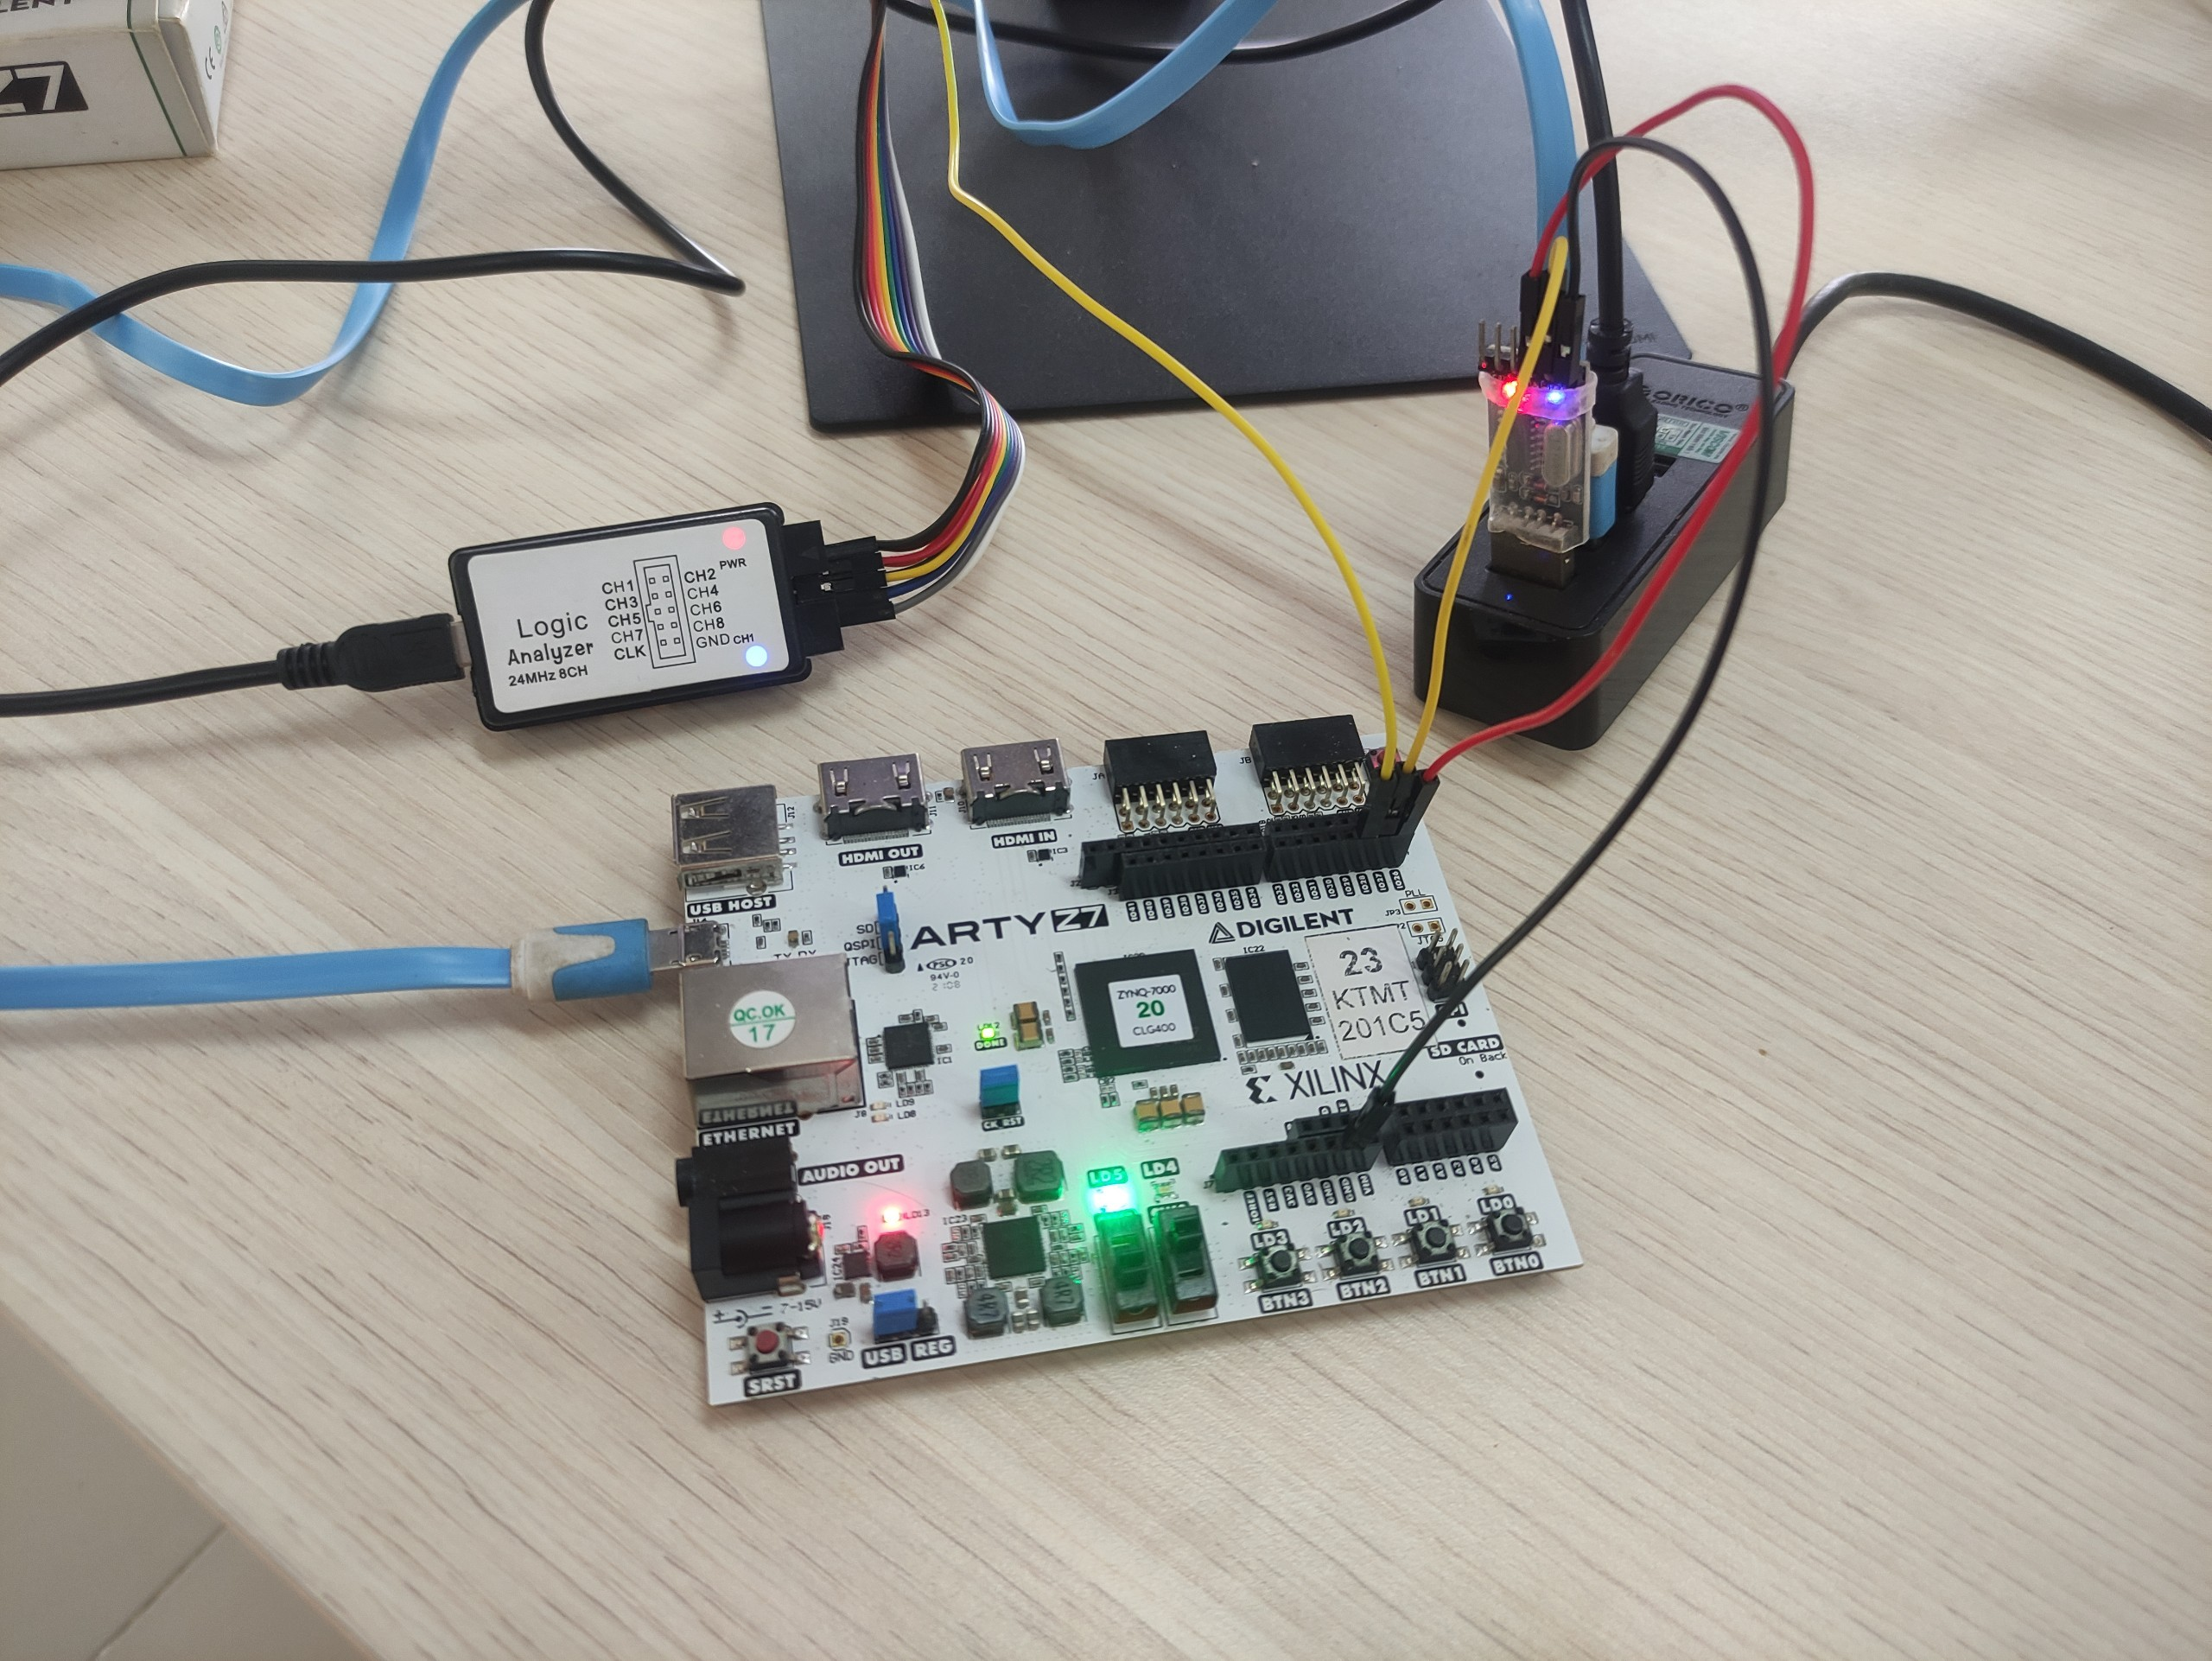
\includegraphics[width=0.9\linewidth]{2_co_so_ly_thuyet/image/uart.png} 
        \caption{Minh họa chân kết nối truyền nhận dữ liệu UART}
        \label{fig:uart_connection}
    \end{figure}

    \begin{figure}[H]
        \centering
        \includegraphics[width=0.8\linewidth]{2_co_so_ly_thuyet/image/uart2.png} 
        \caption{Chuyển đổi dữ liệu song song thành nối tiếp và ngược lại trong UART}
        \label{fig:uart_connection}
    \end{figure}



    \subsubsection{Cấu trúc khung dữ liệu (Data Frame)}
    Do không có xung nhịp đồng bộ, UART sử dụng các bit điều khiển đặc biệt để đánh dấu điểm bắt đầu và kết thúc của một gói tin. Một khung dữ liệu chuẩn bao gồm các thành phần sau:



    \begin{enumerate}
        \item \textbf{Trạng thái nghỉ (Idle State):} Khi không có dữ liệu truyền, đường truyền luôn được giữ ở mức điện áp cao (Logic 1).
        \item \textbf{Start Bit:} Để bắt đầu một phiên truyền, thiết bị phát sẽ kéo đường truyền từ mức cao xuống mức thấp (Logic 0) trong một chu kỳ bit. Bên thu phát hiện cạnh xuống này để bắt đầu quá trình đồng bộ.
        \item \textbf{Data Bits:} Chứa thông tin thực tế cần truyền, thường có độ dài từ 5 đến 9 bit (phổ biến nhất là 8 bit). Theo quy ước, bit có trọng số nhỏ nhất (LSB) được truyền đi trước.
        \item \textbf{Parity Bit (Tùy chọn):} Dùng để kiểm tra lỗi đơn giản. Bit này có thể được cấu hình là chẵn (Even), lẻ (Odd) hoặc không sử dụng (None). Nếu sử dụng, tổng số bit '1' trong gói dữ liệu (bao gồm cả parity) phải thỏa mãn quy tắc chẵn/lẻ đã thiết lập.
        \item \textbf{Stop Bit:} Đánh dấu kết thúc gói tin bằng cách kéo đường truyền về mức cao (Logic 1). Độ dài có thể là 1, 1.5, hoặc 2 bit thời gian. Stop bit đảm bảo đường truyền quay về trạng thái nghỉ để sẵn sàng cho Start bit tiếp theo.
    \end{enumerate}

    \begin{figure}[H]
        \centering
        \includegraphics[width=0.8\linewidth]{2_co_so_ly_thuyet/image/uart_frame.png} 
        \caption{Khung dữ liệu UART}
        \label{fig:uart_frame}
    \end{figure}

    \begin{figure}[H]
        \centering
        \includegraphics[width=0.8\linewidth]{2_co_so_ly_thuyet/image/uart_frame_example.png} 
        \caption{Ví dụ khung dữ liệu UART với 8bit dữ liệu, không parity và 1 stop bit}
        \label{fig:uart_frame}
    \end{figure}

    \subsubsection{Tốc độ Baud (Baud Rate)}
    Vì thiếu xung nhịp đồng bộ, hai thiết bị UART phải thống nhất trước một tốc độ truyền nhận, gọi là Baud Rate (đơn vị: bit/giây - bps).
    \begin{itemize}
        \item Bên phát sẽ đẩy từng bit dữ liệu ra đường truyền với chu kỳ $T = 1/BaudRate$.
        \item Bên thu sẽ lấy mẫu tín hiệu (sample) tại điểm giữa của mỗi chu kỳ bit dự kiến để đọc dữ liệu.
    \end{itemize}
    Theo khuyến cáo kỹ thuật, độ sai lệch tốc độ Baud giữa hai thiết bị không được vượt quá 10\% để đảm bảo dữ liệu được đọc chính xác. Các tốc độ phổ biến thường dùng là 9600, 19200, 115200 bps.


    \subsection{Giao thức truyền thông SPI}

SPI (Serial Peripheral Interface) là chuẩn giao tiếp nối tiếp đồng bộ tốc độ cao, hoạt động ở chế độ song công toàn phần (Full-duplex). Chuẩn này được Motorola giới thiệu vào giữa những năm 1980 và hiện nay đã trở thành tiêu chuẩn công nghiệp để kết nối vi xử lý với các thiết bị ngoại vi như cảm biến, bộ nhớ Flash (SPI Flash), màn hình LCD, hoặc bộ chuyển đổi ADC/DAC.

Khác với UART (bất đồng bộ) hay I2C (bán song công, tốc độ thấp), SPI sử dụng đường xung nhịp riêng biệt và kiến trúc Master-Slave chặt chẽ, cho phép đạt băng thông truyền tải rất cao (có thể lên tới hàng chục MHz).

\subsubsection{Cấu hình tín hiệu vật lý}
Một bus SPI tiêu chuẩn (4-wire mode) bao gồm 4 đường tín hiệu logic kết nối giữa Master và Slave.

% --- VỊ TRÍ CHÈN ẢNH 1: Sơ đồ kết nối Master-Slave ---
\begin{figure}[H]
    \centering
    % Bạn thay tên file ảnh vào dòng dưới
    \includegraphics[width=0.7\linewidth]{2_co_so_ly_thuyet/image/spiwrite.png} 
    \caption{Sơ đồ kết nối tín hiệu chuẩn 4 dây của SPI}
    \label{fig:spi_connection}
\end{figure}

Chức năng các chân tín hiệu bao gồm:
\begin{itemize}
    \item \textbf{SCLK (Serial Clock):} Tín hiệu xung nhịp do Master tạo ra. Toàn bộ quá trình truyền nhận dữ liệu được đồng bộ theo cạnh lên hoặc cạnh xuống của xung này. Slave không được phép tạo xung Clock.
    \item \textbf{MOSI (Master Out Slave In):} Đường truyền dữ liệu từ Master đến Slave.
    \item \textbf{MISO (Master In Slave Out):} Đường truyền dữ liệu từ Slave về Master. Nếu chỉ có Master gửi dữ liệu (ví dụ điều khiển LCD), chân này có thể bỏ qua.
    \item \textbf{CS/SS (Chip Select / Slave Select):} Tín hiệu chọn thiết bị, thường hoạt động ở mức thấp (Active Low). Master kéo chân này xuống 0V để bắt đầu giao dịch với một Slave cụ thể.
\end{itemize}

\subsubsection{Cơ chế hoạt động: Thanh ghi dịch (Shift Register)}
Cốt lõi của giao thức SPI là cấu trúc thanh ghi dịch vòng tròn (Circular Shift Register).

% --- VỊ TRÍ CHÈN ẢNH 2: Cơ chế thanh ghi dịch ---
\begin{figure}[H]
    \centering
    % Bạn thay tên file ảnh vào dòng dưới
    \includegraphics[width=0.9\linewidth]{2_co_so_ly_thuyet/image/spireg.png} 
    \caption{Cơ chế trao đổi dữ liệu dùng thanh ghi dịch trong SPI}
    \label{fig:spi_shift_register}
\end{figure}

Quá trình truyền nhận diễn ra như sau:
\begin{enumerate}
    \item Master và Slave mỗi bên đều có một thanh ghi dịch (thường là 8-bit hoặc 16-bit).
    \item Tại mỗi chu kỳ xung nhịp SCLK:
    \begin{itemize}
        \item 1 bit dữ liệu từ Master được đẩy ra đường MOSI và dịch vào thanh ghi của Slave.
        \item Đồng thời, 1 bit dữ liệu từ Slave được đẩy ra đường MISO và dịch vào thanh ghi của Master.
    \end{itemize}
    \item Sau $N$ chu kỳ xung nhịp (với $N$ là độ rộng dữ liệu), giá trị trong thanh ghi của Master và Slave được trao đổi hoàn toàn cho nhau.
    
\end{enumerate}

\subsubsection{Các chế độ hoạt động (Clock Polarity \& Phase)}
SPI định nghĩa 4 chế độ hoạt động (Modes) dựa trên trạng thái của xung Clock, được quy định bởi hai tham số:
\begin{itemize}
    \item \textbf{CPOL (Clock Polarity):} Trạng thái nghỉ của đường SCLK (0 hoặc 1).
    \item \textbf{CPHA (Clock Phase):} Cạnh lên hoặc xuống của xung dùng để lấy mẫu (Sample) và dùng để thay đổi dữ liệu (Shift).
\end{itemize}

% --- VỊ TRÍ CHÈN ẢNH 3: Giản đồ xung 4 Mode (Lấy từ file Analog Device) ---
% \begin{figure}[H]
%     \centering
%     % Bạn thay tên file ảnh vào dòng dưới
%     \includegraphics[width=0.9\linewidth]{2_co_so_ly_thuyet/image/spi_modes.png} 
%     \caption{Giản đồ thời gian của 4 chế độ hoạt động SPI (CPOL/CPHA)}
%     \label{fig:spi_modes}
% \end{figure}

\begin{figure}[H]
    \centering
    % Bạn thay tên file ảnh vào dòng dưới
    \includegraphics[width=1\linewidth]{2_co_so_ly_thuyet/image/spimode.png} 
    \caption{4 chế độ hoạt động của SPI(CPOL/CPHA)}
    \label{fig:spi_modes}
\end{figure}


\textit{Lưu ý:} Mode 0 và Mode 3 là hai cấu hình phổ biến nhất. Master và Slave phải được cấu hình cùng một Mode để giao tiếp thành công.

\begin{figure}[H]
    \centering
    % Bạn thay tên file ảnh vào dòng dưới
    \includegraphics[width=1\linewidth]{2_co_so_ly_thuyet/image/spimod0.png} 
    \caption{SPI MODE 0 (CPOL=0, CPHA=0), trạng thái SCLK ban đầu ở mức low, dữ liệu được lấy mẫu tại cạnh lên của SCLK và dịch ở cạnh xuống}
    \label{fig:spi_modes}
\end{figure}

\begin{figure}[H]
    \centering
    % Bạn thay tên file ảnh vào dòng dưới
    \includegraphics[width=1\linewidth]{2_co_so_ly_thuyet/image/spimode3.png} 
    \caption{SPI MODE 3 (CPOL=1, CPHA=1), trạng thái SCLK ban đầu ở mức high, dữ liệu được lấy mẫu tại cạnh lên của SCLK và dịch ở cạnh xuống}
    \label{fig:spi_modes}
\end{figure}

\subsubsection{Các mô hình kết nối đa thiết bị}
SPI cho phép một Master giao tiếp với nhiều Slave thông qua hai cấu hình chính:

\textbf{1. Cấu hình Slave độc lập (Independent Slaves):} \\
Master sử dụng các chân CS riêng biệt ($CS_1, CS_2, ...$) cho từng Slave. Đây là cấu hình phổ biến giúp tối ưu băng thông.

\begin{figure}[H]
    \centering
    % Bạn thay tên file ảnh vào dòng dưới
    \includegraphics[width=0.9\linewidth]{2_co_so_ly_thuyet/image/spisingle.png} 
    \caption{Cấu hình Slave độc lập trong SPI}
    \label{fig:spi_modes}
\end{figure}

\textbf{2. Cấu hình Chuỗi (Daisy Chain):} \\
Các Slave được nối tiếp nhau (MISO của Slave này nối vào MOSI của Slave kia). Dữ liệu đi qua chuỗi các thiết bị, giúp tiết kiệm chân điều khiển của Master nhưng làm giảm tốc độ truyền tổng thể.

\begin{figure}[H]
    \centering
    % Bạn thay tên file ảnh vào dòng dưới
    \includegraphics[width=0.9\linewidth]{2_co_so_ly_thuyet/image/spidaisy.png} 
    \caption{Cấu hình Chuỗi (Daisy Chain) trong SPI}
    \label{fig:spi_modes}
\end{figure}

% --- VỊ TRÍ CHÈN ẢNH 4: Cấu hình Daisy Chain vs Independent ---
% \begin{figure}[H]
%     \centering
%     % Bạn thay tên file ảnh vào dòng dưới
%     \includegraphics[width=0.8\linewidth]{2_co_so_ly_thuyet/image/spi_configs.png} 
%     \caption{Hai mô hình kết nối đa thiết bị trong SPI: Độc lập và Chuỗi}
%     \label{fig:spi_configs}
% \end{figure}


    SPI có tốc độ truyền cao nhất so với UART và I2C, phần cứng đơn giản, hỗ trợ Full-duplex. Nhưng tốn nhiều dây tín hiệu, khoảng cách truyền ngắn, không có cơ chế xác nhận lỗi (ACK) như I2C.


\section{Công nghệ FPGA và Quy trình thiết kế}
% Phần này nói về cấu trúc FPGA (LUT, FF, DSP, BRAM) và Flow thiết kế
% File: 2_co_so_ly_thuyet/2.4_cong_nghe_fpga.tex

\subsection{Tổng quan về công nghệ FPGA}
FPGA (Field Programmable Gate Array) là giải pháp vi mạch bán dẫn cho phép tái cấu hình logic sau khi sản xuất, mang lại sự linh hoạt vượt trội so với các thiết kế ASIC cố định. Cấu trúc của FPGA dựa trên một ma trận các khối logic khả trình (Configurable Logic Blocks - CLB) được kết nối với nhau thông qua hệ thống dây dẫn nội bộ linh hoạt (Programmable Interconnects).

Trong lĩnh vực thiết kế SoC và trí tuệ nhân tạo, FPGA mang lại những ưu thế đặc biệt. Khả năng tái cấu hình cho phép các kỹ sư cập nhật thuật toán phần cứng tức thời mà không cần thay đổi bo mạch vật lý. Quan trọng hơn, kiến trúc song song của FPGA rất phù hợp để hiện thực hóa các mảng tính toán Systolic Array trong mạng nơ-ron tích chập (CNN). Điều này giúp giảm thiểu đáng kể rủi ro thiết kế và rút ngắn thời gian đưa sản phẩm ra thị trường (Time-to-market) so với quy trình sản xuất chip ASIC truyền thống.

\subsection{Kiến trúc phần cứng Xilinx 7-Series}
Đề tài được triển khai trên nền tảng kiến trúc \textbf{Xilinx 7-Series}. Cấu trúc phần cứng cơ bản của dòng chip này được hình thành từ hai thành phần tài nguyên cốt lõi:

\subsubsection{Configurable Logic Block (CLB)}
CLB đóng vai trò xương sống của FPGA, chịu trách nhiệm thực hiện các hàm logic tuần tự và tổ hợp. Mỗi CLB chứa các đơn vị nhỏ hơn gọi là Slices, bao gồm các bảng tra 6 đầu vào (\textbf{LUT6}) có thể cấu hình để thực hiện bất kỳ hàm logic nào, cùng với các phần tử nhớ \textbf{Flip-Flop} (FF) để lưu trạng thái và đồng bộ tín hiệu. Ngoài ra, các chuỗi nhớ số học (Carry Chain) tốc độ cao cũng được tích hợp để tối ưu hóa cho các bộ cộng/trừ.


\subsubsection{Bộ nhớ nội BRAM (Block RAM)}
BRAM là các khối bộ nhớ tĩnh (SRAM) dung lượng 36Kb được nhúng rải rác trong FPGA. Chúng đóng vai trò là bộ đệm (Buffer) lưu trữ.

\subsection{Nền tảng phần cứng thực nghiệm}
Quá trình hiện thực hệ thống SoC được tiến hành qua hai giai đoạn thử nghiệm trên hai nền tảng phần cứng khác nhau nhằm đánh giá tính khả thi và tối ưu hóa tài nguyên.

\subsubsection{Giai đoạn 1: Thử nghiệm trên Digilent Arty A7 (Artix-7)}
Ở giai đoạn đầu, nhóm nghiên cứu lựa chọn bo mạch \textbf{Arty A7-100T} (sử dụng chip XC7A100T) làm nền tảng mục tiêu. Tuy nhiên, trong quá trình thiết kế SoC, giới hạn về tài nguyên phần cứng của chip Artix-7 đã trở thành nút thắt cổ chai và giới hạn việc mở rộng. Cụ thể, số dung lượng bộ nhớ BRAM yêu cầu đã vượt quá khả năng cung cấp của chip, dẫn đến việc không thể tổng hợp (Synthesis) thành công thiết kế tối ưu hoặc phải cắt giảm quá nhiều tính năng quan trọng.

\begin{figure}[H]
    \centering
    % Placeholder cho hình quy trình thiết kế
    \includegraphics[width=0.8\linewidth]{2_co_so_ly_thuyet/image/a7.png} 
    \caption{FPGA Arty A7-100T}
    \label{fig:design_flow}
\end{figure}

\subsubsection{Giai đoạn 2: Triển khai trên Xilinx VC707 (Virtex-7)}
Để giải quyết bài toán thiếu hụt tài nguyên và tập trung vào việc kiểm chứng kiến trúc hệ thống (Proof of Concept), đề tài đã chuyển sang sử dụng bo mạch \textbf{Xilinx VC707 Evaluation Kit} (sử dụng chip Virtex-7 XC7VX485T). Đây là dòng FPGA hiệu năng cao với tài nguyên logic và bộ nhớ vượt trội. Việc chuyển đổi sang VC707 cho phép nhóm hiện thực trọn vẹn kiến trúc SoC, tích hợp vi xử lý PicoRV32 và các ngoại vi tốc độ cao mà không bị giới hạn bởi phần cứng.

\begin{figure}[H]
    \centering
    % Placeholder cho hình quy trình thiết kế
    \includegraphics[width=0.9\linewidth]{2_co_so_ly_thuyet/image/vc707.png} 
    \caption{FPGA Xilinx VC707}
    \label{fig:design_flow}
\end{figure}

\begin{table}[H]
    \centering
    \caption{So sánh tài nguyên giữa Arty A7 (Thử nghiệm ban đầu) và VC707 (Triển khai chính thức)}
    \label{tab:fpga_comparison}
    \begin{tabular}{|l|c|c|c|}
        \hline
        \textbf{Tài nguyên} & \textbf{Arty A7 (XC7A100T)} & \textbf{VC707 (XC7VX485T)} & \textbf{Tỷ lệ tăng} \\ \hline
        Logic Cells & 101,440 & 485,760 & $\approx$ 4.8x \\ \hline
        Block RAM & 4.8 Mb & 37 Mb & $\approx$ 7.7x \\ \hline
        DSP Slices & 240 & 2,800& $\approx$ 11.6x \\ \hline
        Transceivers & N/A & GTX (12.5 Gbps) & - \\ \hline
    \end{tabular}
\end{table}
Số liệu từ Bảng \ref{tab:fpga_comparison} cho thấy sự vượt trội về tài nguyên Logic Cells và Block RAM của VC707, đảm bảo không gian rộng lớn cho việc mở rộng quy mô mảng tính toán Systolic Array.

\subsection{Quy trình thiết kế trên Vivado}
Toàn bộ quy trình hiện thực hệ thống SoC được thực hiện trên môi trường \textbf{Xilinx Vivado Design Suite}, tuân thủ luồng thiết kế dựa trên mã nguồn (HDL-based Design Flow) để đảm bảo khả năng kiểm soát chi tiết và tối ưu hóa tài nguyên phần cứng cũng như hướng tói ASIC trong tương lai. \\ 


% \begin{figure}[H]
%     \centering
%     % Placeholder cho hình quy trình thiết kế
%     \includegraphics[width=0.6\linewidth]{2_co_so_ly_thuyet/image/fpga_design_flow.png} 
%     \caption{Quy trình thiết kế vi mạch trên FPGA}
%     \label{fig:design_flow}
% \end{figure}

Quy trình bắt đầu bằng giai đoạn \textbf{Thiết kế (Design Entry)}, trong đó toàn bộ hệ thống được mô tả bằng ngôn ngữ \textbf{Verilog HDL}. Thay vì sử dụng công cụ thiết kế dạng sơ đồ khối (IP Integrator), các thành phần lõi như PicoRV32, hệ thống Bus, khối Accelerator, khối DMA và các khối ngoại vi như UART, SPI, OSPI, I2C, DVP,... được kết nối trực tiếp thông qua kỹ thuật khởi tạo module (Module Instantiation) bên trong một tập tin thiết kế đỉnh (Top-level Module). Sau khi hoàn tất mã nguồn, hệ thống trải qua bước \textbf{Mô phỏng (Simulation)} hành vi bằng Testbench để kiểm chứng tính đúng đắn của logic trước khi đi vào \textbf{Tổng hợp (Synthesis)} để chuyển đổi mã RTL thành danh sách lưới cổng (Netlist). Giai đoạn quan trọng tiếp theo là \textbf{Hiện thực (Implementation)}, bao gồm việc sắp xếp linh kiện (Place) và đi dây (Route) trên chip thực tế, quyết định tần số hoạt động tối đa (Fmax) của hệ thống. Cuối cùng, công cụ sẽ thực hiện \textbf{Tạo Bitstream} (tệp nhị phân .bit) để nạp cấu hình xuống bo mạch FPGA VC707, hoàn tất quy trình thiết kế phần cứng.
% \section{Tổng quan về Trí tuệ nhân tạo và Mạng nơ-ron tích chập}
% % Phần này nói về cấu trúc FPGA (LUT, FF, DSP, BRAM) và Flow thiết kế
% \input{2_co_so_ly_thuyet/2.5_CNN.tex}

\chapter{Công trình nghiên cứu liên quan kiến trúc bộ gia tốc CNN}
\section{Kiến trúc tham chiếu: Hệ thống Eyeriss}Để giải quyết bài toán tối ưu hóa năng lượng cho các mạng nơ-ron tích chập (CNN), kiến trúc Eyeriss (Chen et al., 2017) \cite{chen2017eyeriss} tập trung vào việc cực tiểu hóa chi phí di chuyển dữ liệu thông qua thiết kế phần cứng chuyên biệt và phân cấp bộ nhớ hiệu quả. Hệ thống bao gồm chip tăng tốc kết nối với DRAM ngoại vi qua giao diện bất đồng bộ, cho phép tách biệt miền xung nhịp tính toán và giao tiếp. Trung tâm của kiến trúc là mảng $12 \times 14$ phần tử xử lý (PE) hoạt động độc lập, mỗi PE sở hữu bộ nhớ đệm cục bộ (Scratchpads - Spads) để lưu trữ trọng số, dữ liệu đầu vào và các tổng riêng. Thiết kế này tạo nên mô hình phân cấp bộ nhớ bốn mức, từ DRAM, Global Buffer, Inter-PE đến Spads, giúp khai thác tối đa tính cục bộ của dữ liệu.Đóng vai trò trung chuyển là bộ đệm toàn cục (Global Buffer) dung lượng 108KB, giúp giảm thiểu các truy cập bộ nhớ ngoài tốn kém. Hệ thống sử dụng mạng kết nối trên chip (NoC) tùy biến gồm Mạng đầu vào (GIN) hỗ trợ multicast và Mạng đầu ra (GON). Điểm đặc biệt của Eyeriss là luồng dữ liệu "Row Stationary" (RS), cho phép tái sử dụng dữ liệu hiệu quả ngay tại các bộ nhớ cục bộ trong từng PE, từ đó tối ưu hóa công suất tiêu thụ tổng thể.

\section{Kiến trúc tham chiếu: Bộ tăng tốc Pixel-Level Fully Pipelined}Nhằm khắc phục nhược điểm về độ trễ và thông lượng của các kiến trúc truyền thống xử lý theo lớp (layer-by-layer), Li và cộng sự (2025) \cite{li2025pixel} đã đề xuất kiến trúc đường ống toàn phần ở cấp độ pixel (Pixel-Level Fully Pipelined). Thay vì yêu cầu bộ nhớ đệm lớn để lưu trữ bản đồ đặc trưng giữa các lớp, kiến trúc này triển khai toàn bộ mạng nơ-ron thành chuỗi nối tiếp, cho phép luồng pixel được xử lý liên tục từ đầu vào đến đầu ra. Quy trình xử lý dựa trên chiến lược "pixel-by-pixel", trong đó mỗi lớp tính toán tích hợp ba thành phần chính: bộ chọn kênh (MUX), bộ đệm chỉnh lưu (Rectified FIFO) và đơn vị tính toán (CU). Cụ thể, MUX và Rectified FIFO chịu trách nhiệm trích xuất, đồng bộ và chuẩn hóa dữ liệu cửa sổ trượt từ luồng đầu vào để đảm bảo tính liên tục cho đường ống.Tại đơn vị tính toán (CU), hệ thống thực hiện các phép nhân chập song song và áp dụng kỹ thuật ghép kênh theo thời gian (Time-Division Multiplexing). Kỹ thuật này dựa trên các tham số "Initial Sparsity" (IS) và "Pooling Sparsity" (PS), cho phép tái sử dụng tài nguyên DSP cho nhiều tác vụ trong cùng một chu kỳ xung nhịp. Về mặt lưu trữ, toàn bộ trọng số và bias dạng 8-bit fixed-point được lưu trực tiếp trên các khối BRAM nội bộ đặt cạnh đơn vị xử lý. Thiết kế này loại bỏ hoàn toàn việc truy cập DRAM trong quá trình suy luận, giúp giảm độ trễ xuống dưới mức mili-giây và tối đa hóa hiệu quả năng lượng.

\section{Kiến trúc tham chiếu: Tăng tốc CNN trên FPGA dựa trên OpenCL}Zhang và Li (2017)\cite{zhang2017opencl} đã đề xuất một giải pháp tăng tốc CNN sử dụng ngôn ngữ OpenCL nhằm cân bằng giữa hiệu năng phần cứng và tính linh hoạt trong lập trình. Hệ thống vận hành theo mô hình tính toán dị thể, bao gồm một CPU chủ (Host) điều khiển luồng chương trình và FPGA (Device) thực thi các tác vụ tính toán chuyên sâu. Để giải quyết nút thắt về băng thông bộ nhớ, nhóm tác giả xây dựng "Mô hình phân tích cân bằng" (Balance Analysis Model) giúp định lượng mối tương quan giữa năng lực tính toán và băng thông, từ đó xác định cấu hình tài nguyên tối ưu để thông lượng không bị giới hạn bởi tốc độ truy xuất Global Memory.Hiệu năng hệ thống được nâng cao nhờ thiết kế kernel OpenCL tối ưu. Cụ thể, các kernel được thiết kế dạng đường ống sâu (deep pipelining) để thực thi song song các chỉ lệnh tích chập. Đồng thời, hệ thống quản lý bộ nhớ phân cấp bằng cách tận dụng tối đa Local Memory/BRAM để lưu đệm các bản đồ đặc trưng và trọng số, giảm thiểu truy cập bộ nhớ ngoài (Off-chip Memory). Các kỹ thuật tối ưu hóa vòng lặp như trải phẳng (loop unrolling) và chia nhỏ dữ liệu (loop tiling) cũng được áp dụng triệt để. Kết quả thực nghiệm trên Altera Arria 10 cho thấy kiến trúc đạt hiệu suất 866 GOPS và hiệu quả năng lượng vượt trội so với các thiết kế RTL truyền thống.

\section{Kiến trúc tham chiếu: Hệ thống xử lý dị thể trên nền tảng RISC-V cho IoT}Hướng đến các ứng dụng IoT với ràng buộc khắt khe về tài nguyên, Liu và cộng sự (2020) \cite{liu2020riscv} đề xuất kiến trúc xử lý dị thể kết hợp giữa lõi CPU RISC-V nhúng và khối tăng tốc phần cứng CNN chuyên biệt. Mô hình đồng thiết kế phần cứng/phần mềm này phân chia trách nhiệm rõ ràng: CPU RISC-V đóng vai trò bộ xử lý đa dụng, quản lý luồng chương trình và các tác vụ tiền/hậu xử lý ở tần số thấp (20 MHz) để tiết kiệm năng lượng nền.Trong khi đó, khối CNN Accelerator đảm nhận các phép toán chuyên sâu ở tần số cao hơn (100 MHz) nhằm đảm bảo thông lượng. Giao tiếp giữa hai thành phần được thực hiện qua cơ chế "lệnh vĩ macro" (macro instructions), cho phép CPU cấu hình và kích hoạt Accelerator xử lý trọn vẹn các lớp mạng phức tạp mà không cần can thiệp liên tục. Kiến trúc này minh chứng cho tính hiệu quả khi kết hợp sự linh hoạt của tập lệnh mở RISC-V với hiệu năng xử lý song song của các bộ tăng tốc miền cụ thể (domain-specific accelerators).

\section{Kiến trúc tham chiếu: Bộ tăng tốc luồng cấu hình lại (RSA) cho IoT}Du và cộng sự (2017) \cite{du2017rsa} giới thiệu kiến trúc "Reconfigurable Streaming Architecture" (RSA) dành cho các thiết bị IoT, với đặc điểm cốt lõi là khả năng xử lý dữ liệu theo luồng liên tục (streaming). RSA loại bỏ hoàn toàn nhu cầu lưu trữ các bản đồ đặc trưng trung gian vào DRAM, giúp giảm đáng kể độ trễ và năng lượng tiêu thụ. Thay vì lưu trữ toàn bộ khung hình, hệ thống sử dụng các bộ đệm dòng (Line Buffers) dựa trên FIFO để lưu tạm thời các dòng pixel đầu vào cần thiết cho cửa sổ trượt, giúp tối ưu hóa tài nguyên bộ nhớ on-chip.Các phép tính tích chập, pooling và kích hoạt được thực hiện bởi các Đơn vị tính toán cấu hình lại, kết nối qua mạng lưới chuyển mạch tùy biến. Thiết kế này cho phép định tuyến luồng dữ liệu động để hỗ trợ đa dạng kích thước kernel (như $3\times3$, $1\times1$) mà không cần thay đổi phần cứng vật lý. Đồng thời, băng thông bộ nhớ ngoài được dành riêng cho việc nạp trọng số, hoặc trọng số được lưu trực tiếp trên SRAM nội bộ nhằm tối đa hóa hiệu quả năng lượng cho toàn hệ thống.